\section{Introduction}
\label{sec:introduction}

\paragraph{} The objective of this laboratory assignment is to design an Audio Amplifier, this is a device that can increase the power of a signal so it can be transmited (in our case a voltage that varies with time).

\paragraph{} The architecture chosen for the lab is the one detailed bellow.

\begin{figure}[h]
	\centering
	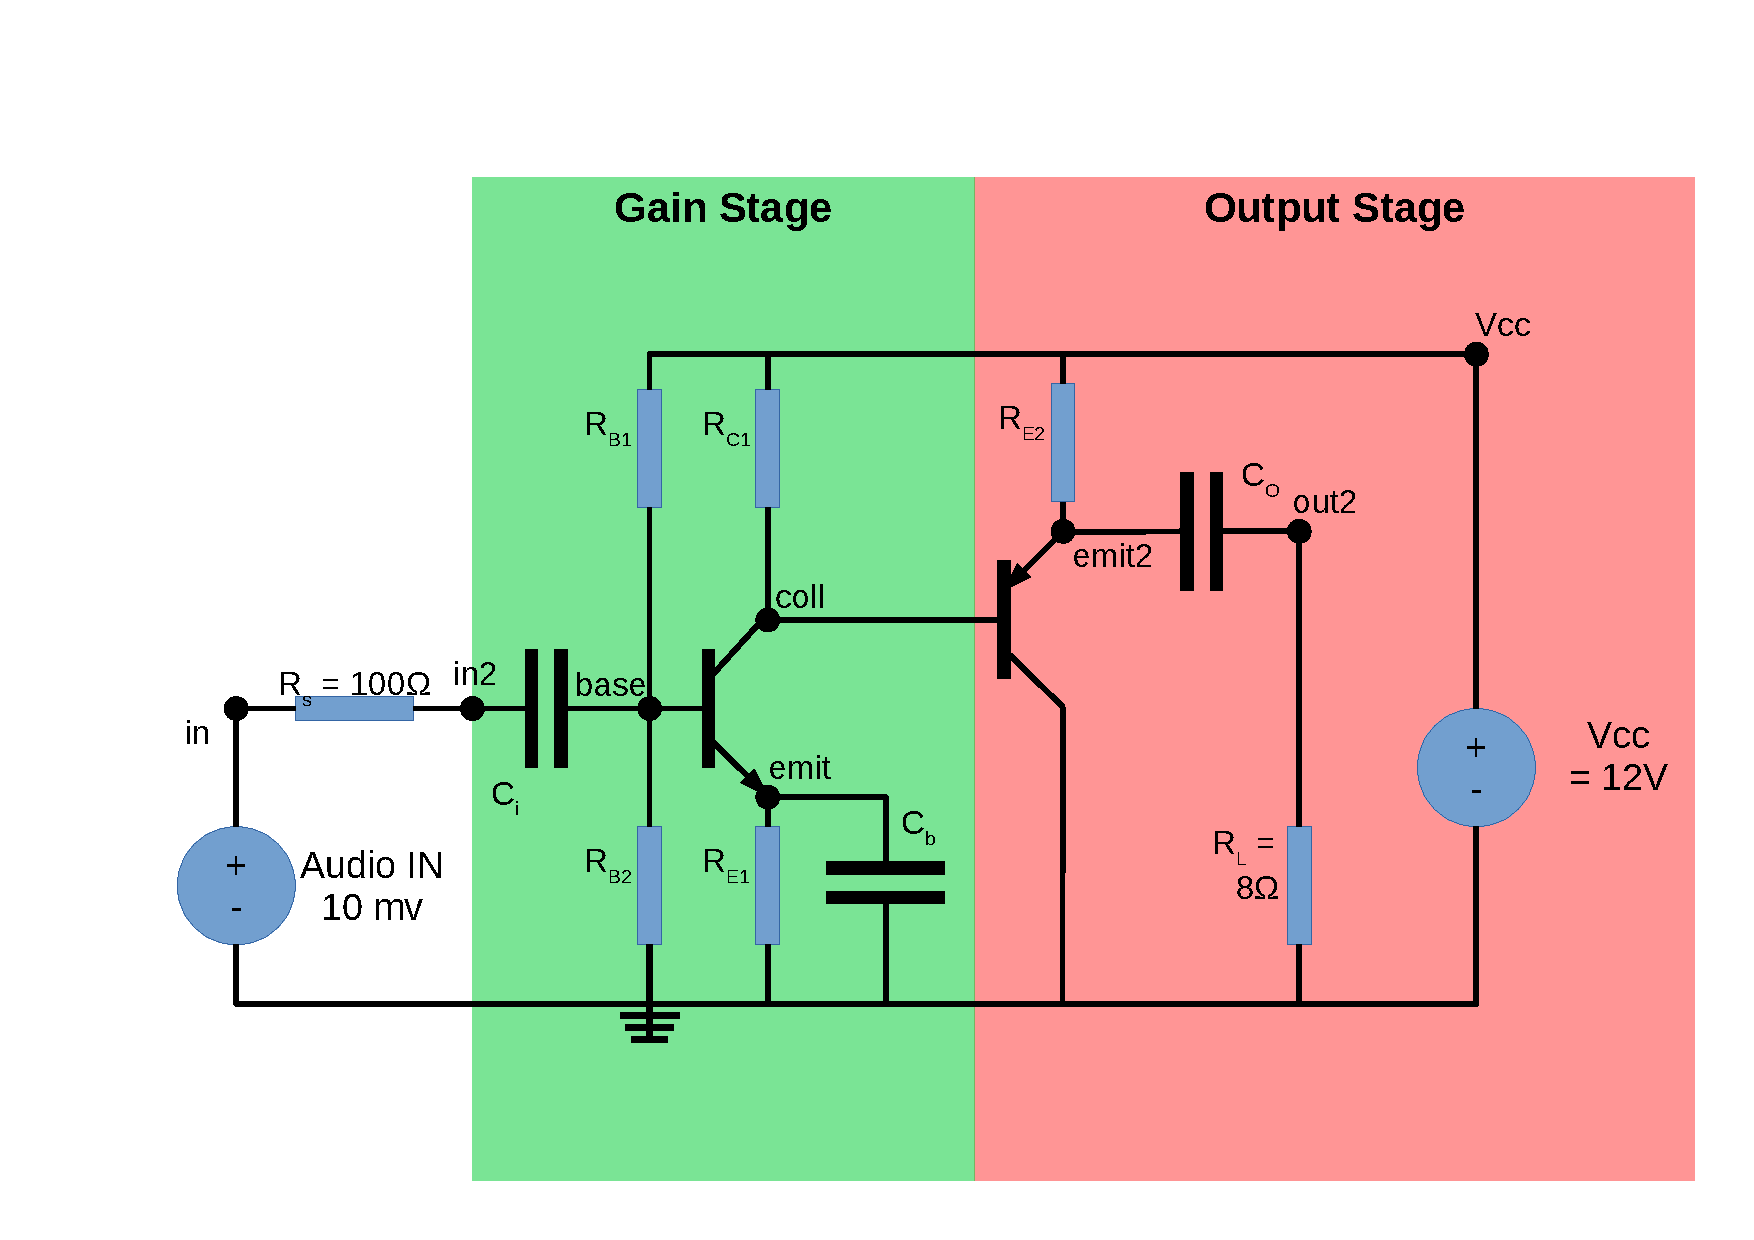
\includegraphics[width=0.9\linewidth]{./Circuit.pdf}
	\caption{T2 RC circuit.}
	\label{fig:rc}
\end{figure}

\paragraph{} It can be decomposed in two main stages: the Gain Stage (in green) and the Output Stage (in red).

\paragraph{} In the Gain Stage the original signal will be amplified. However, this amplified signal is not apropriate to be connected to our load (the speaker) due to it's high impedance.

\paragraph{} Therefore, the signal goes through the Output Stage, that, due to its lowed impedance, makes the signal suitable to be conected to the speaker (which is connected in series).

\paragraph{} To perform the Theoretical Analysis we will look into the Gain and Output Stages separatelly.

\paragraph{} In Section 2 we will perform the Theortetical Analysis of the circuit, determining the operating point gain, impedances and frequency response.

\paragraph{} In Section 3 we will obtain the simulation results to perform the Simulation Analysis.

\paragraph{} To finish, we will draw our comparisons in Section 4 and lay our conclusions, looking into any possible differences and determining it's causes.

\paragraph{} In the table bellow we list the numerical values of the components used.

\begin{table}[h]
  \centering
  \begin{tabular}{|l|r|}
    \hline    
    {\bf Name} & {\bf Values} \\ \hline
    VT& 0.025000 V \\ \hline 
BFN& 178.700000 \\ \hline 
VAFN& 69.700000 V \\ \hline 
VBEON& 0.700000 V \\ \hline 
BFP& 227.300000 \\ \hline 
VAFP& 37.200000 V \\ \hline 
VEBON& 0.700000 V \\ \hline 
VCC& 12.000000 V \\ \hline 
RB1& 55.000000 kOhm \\ \hline 
RB2& 20.000000 kOhm \\ \hline 
RE1& 200.000000 Ohm \\ \hline 
RC1& 800.000000 Ohm \\ \hline 
RE2& 50.000000 Ohm \\ \hline 
$C_{input}$& 0.100000 mF \\ \hline 
$C_{bypass}$& 2.500000 mF \\ \hline 
$C_{output}$& 1.500000 mF \\ \hline 
 
  \end{tabular}
  \caption{Values of components used in our analysis and simulation.}
  \label{tab:data}
\end{table}


\clearpage
